
\documentclass[sn-basic]{sn-jnl}

%% Required by sn-jnl class (footnote hooks, colors)
\usepackage{xcolor}
\usepackage{manyfoot}

%% Standard packages
\usepackage{graphicx}
\usepackage{booktabs}
\usepackage{multirow}
\usepackage{amsmath,amssymb}
\usepackage{enumitem}
\usepackage{algorithm}
\usepackage{algpseudocode}
\usepackage{url}

%% Local macros
\newcommand{\model}{V-CHIMERA}
\newcommand{\envname}{CyberCrisisGym-J}

\title[\model{}]{\model{}: Verified Coupled Human--Information--Machine Incident Response for Misinformation-Aware Cyber Defense}

%% NOTE (double-anonymous review):
%% Provide author names/affiliations in the submission system metadata.
%% Keep the manuscript anonymized.
\author*[1]{Anonymous Author(s)}
\affil[1]{Anonymous affiliation(s)}

\abstract{Cyber incidents increasingly unfold as cyber--social crises: misinformation, speculation, and opportunistic scams can suppress reporting and compliance, amplifying operational harm and undermining trust in official channels. We introduce \model{}, a verified multi-agent framework that couples incident response with crisis communication under explicit protocol constraints. The framework coordinates two decision-makers---a cyber response policy and a messaging policy conditioned on latent public sentiment (misbelief, trust, uncertainty, polarization)---within a coupled cyber--social environment. A runtime communication \emph{shield} enforces conservative governance rules (evidence-gated debunking, uncertainty labeling, disclosure limits, and cooldowns), guaranteeing zero executed protocol violations while logging attempted violations and interventions for auditability. We instantiate \model{} in \envname{}, which combines an attack-graph incident simulator with a multi-platform social-network agent-based model (communities, bots, moderation), and evaluate three crisis scenarios (ransomware rumor, outage rumor, and exfiltration scam) with targeted-messaging and coupling ablations. Results show that verified enforcement eliminates unsafe communications and that coupling yields scenario-dependent trade-offs: in outage-rumor, coupling with targeting reduces misbelief and increases trust relative to a shielded sequential baseline at modest cyber cost, whereas in ransomware-rumor and exfiltration-scam, naive coupling can increase cyber harm, highlighting the need to calibrate coupling functions to operational context. A sensitivity analysis further shows that the marginal value of verified communication grows with stronger cyber-to-social coupling and weaker platform moderation.}

\keywords{cyber incident response; misinformation; crisis communication; social cybersecurity; multi-agent systems; runtime enforcement; safety constraints}

\begin{document}

\maketitle

\section{Introduction}
Cyber incidents are rarely confined to technical containment. Ransomware disruptions, service outages, and data-exfiltration events are routinely accompanied by rumor, speculation, coordinated disinformation, and opportunistic scams, all of which can shape public behavior and constrain operational response. This aligns with the literature on \emph{social cybersecurity}, which emphasizes that human behavior and online information flows are integral to cybersecurity outcomes \citep{carley2020social,mulahuwaish2025survey}.

From an incident-response perspective, misinformation can \emph{increase} harm by suppressing reporting of indicators, discouraging compliance with mitigation guidance, overwhelming helpdesks, or redirecting victims to follow-on phishing and fraud. Conversely, crisis communications are safety-critical: overconfident debunks, premature attribution, or over-disclosure can cause irreversible damage (panic, legal exposure, privacy breaches, or loss of trust). Despite these bidirectional dependencies, autonomous cyber-defense benchmarks typically study containment in isolation (e.g., enterprise-defense simulation gyms \citep{baillie2020cyborg,kunz2023multiagent}), while misinformation research often evaluates interventions without closed-loop operational feedback \citep{lazer2018science,vosoughi2018spread,kozyreva2024toolbox,lewandowsky2021inoculation,ng2021platform}.

This paper asks how to design socio-technical decision systems that \emph{jointly} manage incident response and public communication under explicit governance constraints. We focus on three research questions:
\begin{enumerate}[leftmargin=*]
  \item \textbf{RQ1:} When public sentiment affects operational dynamics, does coupling sentiment into incident-response decision-making improve outcomes under misinformation?
  \item \textbf{RQ2:} When messaging capacity is limited and susceptibility is heterogeneous, do targeted counter-messaging strategies better reduce misbelief and preserve trust than non-targeted baselines?
  \item \textbf{RQ3:} Can runtime protocol enforcement eliminate unsafe communications (zero executed violations) while preserving effectiveness?
\end{enumerate}

\subsection{Contributions}
We make four contributions:
\begin{enumerate}[leftmargin=*]
  \item \textbf{Problem formulation.} We formalize misinformation-aware incident response as a constrained partially observable stochastic game (C-POSG) with a coupled cyber--social state and a safety-constrained communication channel.
  \item \textbf{Verified architecture.} We introduce \model{}, a modular two-agent decision architecture coupling cyber operations and crisis communication through a shared belief-state estimate and an explicit coupling function.
  \item \textbf{Runtime enforcement for communication safety.} We adapt shielding to crisis messaging by enforcing protocol predicates at runtime, guaranteeing zero executed protocol violations and producing auditable intervention logs.
  \item \textbf{Reproducible testbed and evaluation.} We instantiate the framework in \envname{} and report scenario-based experiments with ablations and sensitivity analysis in a fully scriptable pipeline.
\end{enumerate}

\section{Background and related work}
We situate \model{} at the intersection of misinformation dynamics, social cybersecurity, multi-agent decision-making, and safe runtime enforcement.

\subsection{Misinformation dynamics and interventions}
False information can spread faster and farther than corrections in online networks \citep{vosoughi2018spread,lazer2018science}. Susceptibility is shaped by attention and reasoning constraints \citep{pennycook2019lazy}. Interventions such as debunking, prebunking/inoculation, accuracy prompts, and platform moderation can reduce belief and sharing of falsehoods \citep{kozyreva2024toolbox,lewandowsky2021inoculation,ng2021platform}. In crisis settings, however, interventions are embedded in operational feedback loops: public compliance and reporting affect incident evolution, and cyber events (confirmed breach, service loss) shift beliefs and trust. This motivates closed-loop evaluation rather than isolated intervention assessment.

\subsection{Opinion dynamics and social-network models}
Opinion dynamics models provide mechanistic abstractions for belief evolution under social influence, including DeGroot consensus \citep{degroot1974reaching} and bounded confidence \citep{hegselmann2002opinion}. We adopt an agent-based modeling approach because cyber--social crises are heterogeneous, multi-platform, and adversarially manipulated (bots and coordinated campaigns). The \envname{} social backend exposes interpretable parameters (susceptibility, correction efficacy, moderation strength) and yields macro metrics including misbelief, trust, uncertainty, and polarization.

\subsection{Social cybersecurity and cyber--social coupling}
Social cybersecurity argues that attackers exploit both technical and social channels \citep{carley2020social,mulahuwaish2025survey}. In incident response, public behavior affects detection (e.g., user-reported phishing) and mitigation (compliance with patching and isolation guidance). Our framework encodes these dependencies via an explicit coupling function and evaluates policy trade-offs under different coupling regimes.

\subsection{Multi-agent systems and coordination under uncertainty}
Multi-agent systems provide tools for distributed decision-making and coordination under uncertainty \citep{wooldridge2009introduction,jennings2001agentbased,rahwan2019machine,tambe2011security}. In cyber defense, simulation environments such as CybORG \citep{baillie2020cyborg} and CyberBattleSim \citep{kunz2023multiagent} enable evaluation of autonomous defenders, but typically omit the public communication dimension and associated safety constraints.

\subsection{Safe decision-making and shielding}
Runtime shielding can prevent unsafe actions during learning or deployment by enforcing hard constraints on the executed policy \citep{alshiekh2018safe,koenighofer2024shields}. We adapt this concept to \emph{communication safety} in cyber crises: unsafe actions correspond to protocol violations such as over-claiming without evidence, over-disclosure of sensitive details, or harmful user instructions. Because communications can create irreversible harm, hard constraints are appropriate.

\section{Research design}
We follow a design science perspective \citep{hevner2004designscience,peffers2007dsrm}, treating \model{} as a socio-technical artifact for cyber crisis management in online information environments. Design science is appropriate because the contribution is prescriptive: we build a verified decision architecture and evaluate its utility under controlled conditions.

The design objectives are: (i) explicitly model cyber--social coupling; (ii) support targeted counter-messaging under heterogeneous diffusion; (iii) enforce non-negotiable communication protocol constraints via runtime enforcement; and (iv) provide transparent evaluation and artifact transparency. We evaluate \model{} in \envname{} using scenario-based simulation, ablations (no coupling, no targeting), and baseline pipelines with and without shielding.

\section{Problem formulation}
We model a misinformation-aware cyber crisis as a constrained partially observable stochastic game.

\subsection{State, actions, and observations}
Let $s_t = (s^C_t, s^S_t)$ denote the joint state at time $t$, comprising cyber state $s^C_t$ (e.g., compromise status and service availability) and social state $s^S_t$ (distribution of beliefs and trust across a population and platforms). Two decision-makers act at each step: a cyber agent with action $a^C_t \in \mathcal{A}^C$ (operational response such as isolation, patching, restoration, and detection), and a communication agent with action $a^M_t \in \mathcal{A}^M$ (public messaging such as status updates, advisories, or rumor corrections).

Observations are partial: $o^C_t$ captures noisy cyber telemetry, while $o^S_t$ captures noisy social signals (polls, sentiment summaries, or sampled posts). Agents may share a belief state $b_t \approx p(s_t \mid o_{\le t}, a_{<t})$.

\subsection{Objectives and constraints}
We seek to reduce cyber harm while stabilizing sentiment:
\begin{align}
R_t &= -\alpha \cdot H(s^C_t) - \beta \cdot M(s^S_t) + \gamma \cdot T(s^S_t),
\end{align}
where $H$ is cyber harm (e.g., service loss and exfiltration), $M$ is misbelief, and $T$ is trust. Communication safety constraints are encoded as protocol predicates $g_k(s_t,a^M_t) \le 0$. A runtime shield enforces these constraints by editing unsafe actions into safe alternatives.

\section{\model{} framework}
Figure~\ref{fig:arch} summarizes the architecture.

\begin{figure}[t]
  \centering
  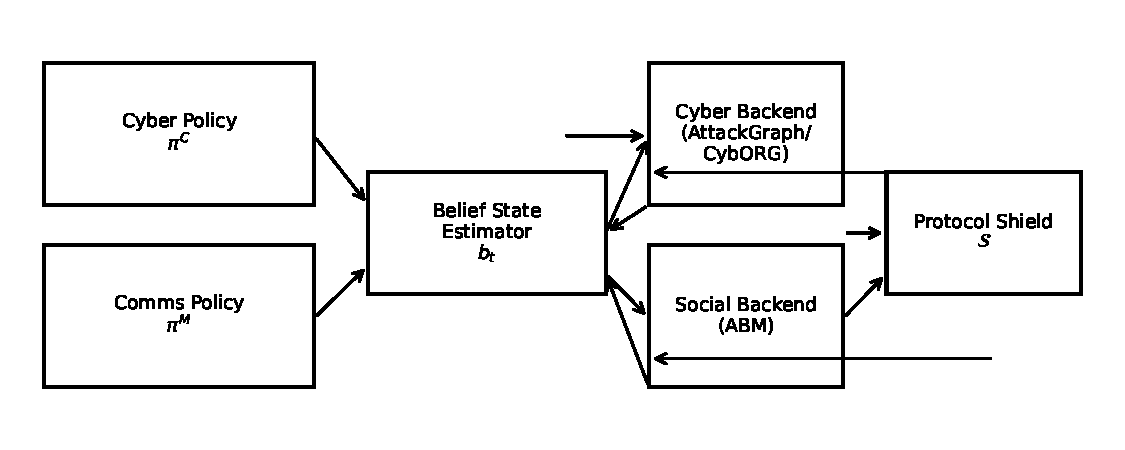
\includegraphics[width=0.95\linewidth]{figures/fig_architecture_gray.pdf}
  \caption{System overview. Two cooperating decision-makers select cyber operations and public communications. Communication actions are filtered by a runtime protocol shield that guarantees zero executed protocol violations while logging attempted violations and interventions. A coupled cyber--social environment (\envname{}) models bidirectional feedback between operational state and social dynamics.}
  \label{fig:arch}
\end{figure}

\subsection{Cyber policy}
The cyber policy $\pi^C(a^C_t \mid o^C_t, b_t)$ selects operational actions. In this work we instantiate $\pi^C$ using a rule-based incident-response controller with configurable aggressiveness and prioritization (patch versus isolate versus restore). This provides a transparent baseline suitable for ablation and reproducibility; the framework is compatible with learned policies (e.g., MARL) in future work.

\subsection{Communication policy with targeting}
The communication policy $\pi^M(a^M_t \mid o^S_t, b_t)$ proposes messaging actions conditioned on the estimated sentiment state. We distinguish targeted messaging, which focuses interventions on communities with high misbelief or low trust, from non-targeted broadcast messaging. Targeting is implemented via a community-level risk estimator that ranks subpopulations by misinformation exposure and susceptibility.

\subsection{Coupling function}
A coupling function $\Phi$ maps social macro-state to cyber-relevant quantities. In \envname{}, compliance affects the effectiveness of operational mitigation (e.g., patch adoption and isolation adherence) and reporting affects detection probability (e.g., user-reported phishing). Trust moderates how strongly official messages shift beliefs. Conversely, cyber events (service loss, confirmed compromise) inject narrative shocks that perturb social dynamics, capturing how technical realities shape online discourse.

\section{Communication protocol and runtime shield}
A central design principle in \model{} is that crisis communications are safety-critical actions. Unlike many cyber actions, harmful public statements can cause irreversible damage. We therefore represent communication governance as a protocol and enforce it at runtime.

\subsection{Protocol as constraint predicates}
Let $a^M_t$ be a communication action parameterized by an intent (e.g., status update, rumor correction), targeting scope (broadcast versus communities), and certainty level. We define safety predicates $\{g_k\}_{k=1}^K$ such that a message is safe iff
\begin{equation}
\forall k,\quad g_k(s_t, a^M_t) \le 0.
\end{equation}
In the artifact, $g_k$ is implemented as a lightweight rule set checking for over-claiming (high certainty with low detection confidence), over-disclosure (naming specific assets or unverified root causes), harmful instructions, and contradictions with earlier official statements.

\subsection{Shield operation}
Given a proposed action $a^M_t$ from the comms policy, the shield computes
\begin{equation}
\tilde a^M_t = \mathcal{S}(a^M_t, s_t),
\end{equation}
where $\tilde a^M_t = a^M_t$ if safe; otherwise $\tilde a^M_t$ is the nearest safe alternative under a discrete edit distance (e.g., downgrade certainty, switch to a hold statement, or remove targeting). This follows the ``optimize under soft objectives, enforce hard constraints at runtime'' principle \citep{alshiekh2018safe,koenighofer2024shields}.

\subsection{End-to-end step algorithm}
Algorithm~\ref{alg:step} summarizes the closed-loop interaction.

\begin{algorithm}[t]
\caption{\model{} closed-loop step (single episode)}
\label{alg:step}
\begin{algorithmic}[1]
\State Initialize environment state $s_0$, observations $o_0$, and belief state $b_0$
\For{$t=0,\dots,T-1$}
  \State Observe $(o^C_t, o^S_t)$
  \State Update belief $b_t \leftarrow \textsc{Estimate}(b_{t-1}, o_t)$
  \State Propose cyber action $a^C_t \sim \pi^C(\cdot \mid o^C_t, b_t)$
  \State Propose comms action $a^M_t \sim \pi^M(\cdot \mid o^S_t, b_t)$
  \State Enforce protocol $\tilde a^M_t \leftarrow \mathcal{S}(a^M_t, s_t)$
  \State Step environment $(s_{t+1}, o_{t+1}) \leftarrow \mathcal{P}(s_t, a^C_t, \tilde a^M_t)$
  \State Log metrics (harm, misbelief, trust, violations, edits)
\EndFor
\end{algorithmic}
\end{algorithm}

\section{\envname{} coupled cyber--social testbed}
\envname{} couples (i) a cyber incident simulator and (ii) a multi-platform social-network agent-based model, enabling closed-loop evaluation.

\subsection{Cyber backend}
The default cyber backend is an attack-graph simulator with stochastic attacker progression and defender actions under resource constraints. The defender can isolate nodes, patch vulnerabilities, restore services, and allocate detection effort. Cyber harm aggregates availability loss, compromise spread, and exfiltration proxies. While simplified relative to a real enterprise network, the backend supports heterogeneous assets, multiple attacker objectives, and action costs, enabling systematic ablations.

\subsection{Social backend}
The social backend simulates a population partitioned into communities and exposed to multiple platforms. Individuals update beliefs based on peer exposure, bot-driven misinformation injection, official communication, and platform moderation (removal and labeling). The model outputs macro metrics---misbelief, trust, uncertainty, and polarization---which define the sentiment state coupled to cyber dynamics.

\subsection{Calibration}
Agent-based models can exhibit degenerate regimes (immediate consensus or total fragmentation). We therefore include a calibration routine that searches parameter space to match stylized crisis-regime target intervals. Table~\ref{tab:calibration} reports one representative calibration instance from our run; it yields a conservative baseline with trust slightly below the target interval, stressing the communication component.

\begin{table}[t]
\centering
\caption{Example calibration summary for the social ABM (time-averaged crisis-regime metrics).}
\label{tab:calibration}
\small
\begin{tabular}{lccc}
\toprule
Metric & Target range & Calibrated value & Within range? \\
\midrule
Misbelief & [0.20,0.35] & 0.280 & Yes \\
Trust & [0.45,0.65] & 0.396 & No \\
Uncertainty & [0.30,0.55] & 0.385 & Yes \\
Polarization & [0.03,0.12] & 0.032 & Yes \\
\bottomrule
\end{tabular}
\end{table}

\subsection{External backend adapter (optional)}
To support extensibility beyond the default incident simulator, the artifact includes an adapter scaffold for the CybORG enterprise benchmark \citep{baillie2020cyborg,standen2021cyborg,emerson2024cyborgpp}. Because installation and scenario assets vary across systems, we treat transfer experiments as an optional extension and report illustrative transfer diagnostics in Appendix~\ref{app:cyborg}.

\section{Experimental methodology}
\subsection{Scenarios and policies}
We evaluate three crisis scenarios: \emph{ransomware rumor}, \emph{service outage rumor}, and \emph{exfiltration scam}. Each scenario specifies a cyber incident trace distribution, an initial narrative shock, and an attacker misinformation strategy.

We compare six policies:
\begin{itemize}[leftmargin=*]
  \item \textbf{pipeline}: sequential baseline (cyber response + generic comms) with no coupling and no shield.
  \item \textbf{pipeline+shield}: baseline pipeline with protocol enforcement enabled.
  \item \textbf{vchimera}: coupled cyber+comms without shield.
  \item \textbf{vchimera+shield}: full system with protocol enforcement.
  \item \textbf{vchimera-no-coupling+shield}: ablation removing cyber--social coupling.
  \item \textbf{vchimera-no-targeting+shield}: ablation removing targeting (broadcast only).
\end{itemize}

\subsection{Metrics}
We compute time-normalized area-under-curve (AUC) for cyber harm (lower is better), misbelief (lower is better), trust (higher is better), uncertainty (lower is better), and polarization (lower is better). Primary outcomes (cyber harm, misbelief, trust) are reported alongside protocol-safety signals (executed violations and shield edits). Polarization is reported in Appendix~\ref{app:polarization}.

\subsection{Statistical reporting}
Each scenario-policy pair is evaluated over multiple random seeds (see the released configuration files). We report mean and uncertainty intervals as produced by the evaluation scripts and retain raw episode logs for auditability. The artifact additionally provides paired permutation tests across seeds for key comparisons; we summarize these in text rather than reproducing extensive hypothesis-test tables.

\section{Results}
We first report aggregate outcomes and protocol compliance, then examine dynamics and robustness.

\subsection{Main results}
Table~\ref{tab:main} reports the main results across scenarios and policies.

\begin{tableorg}[t]
\centering
\caption{Main results (mean $\pm$ 95\% CI as produced by the artifact scripts). Lower is better for cyber harm, misbelief, and executed protocol violations; higher is better for trust. ``Shield edits'' counts runtime interventions by the communication shield.}
\label{tab:main}
\small
\setlength{\tabcolsep}{3pt}
\resizebox{\textwidth}{!}{
\begin{tabular}{llrrrrr}
\toprule
Scenario & Policy & Cyber harm AUC $\downarrow$ & Misbelief AUC $\downarrow$ & Trust AUC $\uparrow$ & Executed viol. $\downarrow$ & Shield edits \\
\midrule
exfiltration\_scam & pipeline & 2.239 $\pm$ 1.125 & 0.617 $\pm$ 0.218 & 0.200 $\pm$ 0.178 & 137.581 $\pm$ 75.958 & 0.000 $\pm$ 0.000 \\
exfiltration\_scam & pipeline+shield & 2.211 $\pm$ 1.092 & 0.683 $\pm$ 0.247 & 0.201 $\pm$ 0.177 & 0.000 $\pm$ 0.000 & 40.032 $\pm$ 21.165 \\
exfiltration\_scam & vchimera & 2.303 $\pm$ 1.091 & 0.660 $\pm$ 0.269 & 0.276 $\pm$ 0.206 & 46.806 $\pm$ 19.952 & 0.000 $\pm$ 0.000 \\
exfiltration\_scam & vchimera+shield & 2.432 $\pm$ 0.945 & 0.710 $\pm$ 0.230 & 0.202 $\pm$ 0.190 & 0.000 $\pm$ 0.000 & 33.677 $\pm$ 10.719 \\
exfiltration\_scam & vchimera-no-coupling+shield & 2.303 $\pm$ 1.050 & 0.698 $\pm$ 0.240 & 0.193 $\pm$ 0.174 & 0.000 $\pm$ 0.000 & 30.290 $\pm$ 13.292 \\
exfiltration\_scam & vchimera-no-targeting+shield & 2.440 $\pm$ 0.908 & 0.658 $\pm$ 0.236 & 0.198 $\pm$ 0.167 & 0.000 $\pm$ 0.000 & 32.419 $\pm$ 10.804 \\
outage\_rumor & pipeline & 1.128 $\pm$ 0.946 & 0.456 $\pm$ 0.216 & 0.328 $\pm$ 0.188 & 79.065 $\pm$ 70.478 & 0.000 $\pm$ 0.000 \\
outage\_rumor & pipeline+shield & 1.121 $\pm$ 0.935 & 0.505 $\pm$ 0.249 & 0.310 $\pm$ 0.204 & 0.000 $\pm$ 0.000 & 28.516 $\pm$ 24.588 \\
outage\_rumor & vchimera & 1.202 $\pm$ 0.951 & 0.368 $\pm$ 0.182 & 0.472 $\pm$ 0.156 & 33.710 $\pm$ 22.772 & 0.000 $\pm$ 0.000 \\
outage\_rumor & vchimera+shield & 1.232 $\pm$ 0.980 & 0.456 $\pm$ 0.252 & 0.375 $\pm$ 0.235 & 0.000 $\pm$ 0.000 & 24.613 $\pm$ 15.962 \\
outage\_rumor & vchimera-no-coupling+shield & 1.075 $\pm$ 0.890 & 0.493 $\pm$ 0.248 & 0.318 $\pm$ 0.205 & 0.000 $\pm$ 0.000 & 20.129 $\pm$ 14.665 \\
outage\_rumor & vchimera-no-targeting+shield & 1.282 $\pm$ 0.957 & 0.339 $\pm$ 0.179 & 0.356 $\pm$ 0.216 & 0.000 $\pm$ 0.000 & 21.548 $\pm$ 13.069 \\
ransomware\_rumor & pipeline & 1.610 $\pm$ 1.225 & 0.504 $\pm$ 0.215 & 0.290 $\pm$ 0.186 & 93.581 $\pm$ 72.107 & 0.000 $\pm$ 0.000 \\
ransomware\_rumor & pipeline+shield & 1.550 $\pm$ 1.145 & 0.562 $\pm$ 0.250 & 0.281 $\pm$ 0.193 & 0.000 $\pm$ 0.000 & 32.419 $\pm$ 23.632 \\
ransomware\_rumor & vchimera & 1.953 $\pm$ 1.211 & 0.503 $\pm$ 0.216 & 0.383 $\pm$ 0.167 & 42.452 $\pm$ 18.884 & 0.000 $\pm$ 0.000 \\
ransomware\_rumor & vchimera+shield & 2.117 $\pm$ 1.310 & 0.590 $\pm$ 0.243 & 0.279 $\pm$ 0.208 & 0.000 $\pm$ 0.000 & 30.710 $\pm$ 13.806 \\
ransomware\_rumor & vchimera-no-coupling+shield & 1.741 $\pm$ 1.319 & 0.563 $\pm$ 0.254 & 0.276 $\pm$ 0.190 & 0.000 $\pm$ 0.000 & 23.387 $\pm$ 14.308 \\
ransomware\_rumor & vchimera-no-targeting+shield & 2.170 $\pm$ 1.255 & 0.479 $\pm$ 0.207 & 0.265 $\pm$ 0.179 & 0.000 $\pm$ 0.000 & 27.290 $\pm$ 10.463 \\
\bottomrule
\end{tabular}
}
\end{tableorg}

Across scenarios, shielding provides a hard safety guarantee: all shielded policies execute zero protocol violations while producing an auditable edit log (Table~\ref{tab:protocol}). On effectiveness, we observe regime dependence. In \texttt{outage\_rumor}, the shielded coupled system (\texttt{vchimera+shield}) reduces misbelief and increases trust relative to a shielded sequential baseline (\texttt{pipeline+shield}) at a modest cyber-harm increase. In \texttt{ransomware\_rumor} and \texttt{exfiltration\_scam}, the same coupling does not dominate the shielded baseline and can increase cyber harm, underscoring that coupling functions and policy weights must be calibrated to operational context.

To visualize cyber--social trade-offs, Figure~\ref{fig:tradeoff} plots misbelief versus cyber harm for each scenario. The accent marker highlights \texttt{vchimera+shield} against shielded and unshielded baselines.

\begin{figure}[t]
  \centering
  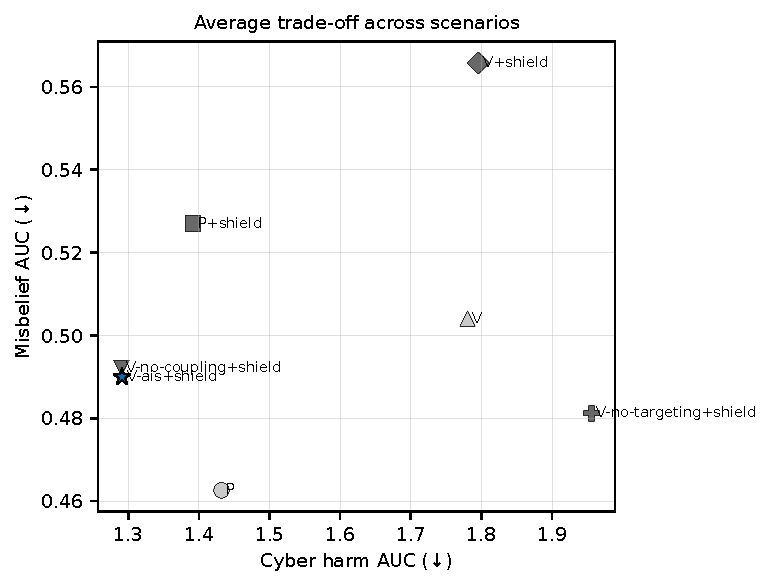
\includegraphics[width=\linewidth]{figures/fig_tradeoff_bw.pdf}
  \caption{Trade-off visualization: misbelief AUC versus cyber-harm AUC (mean and uncertainty bars) across scenarios. Gray markers indicate baselines and ablations; the accent marker highlights the verified coupled system (\texttt{vchimera+shield}).}
  \label{fig:tradeoff}
\end{figure}

\subsection{Protocol compliance}
Table~\ref{tab:protocol} summarizes protocol safety signals.

\begin{table}[t]
\centering
\caption{Protocol compliance (mean $\pm$ 95\% CI). The shield prevents unsafe communication actions from executing.}
\label{tab:protocol}
\small
\setlength{\tabcolsep}{3pt}
\begin{tabular}{llrrr}
\toprule
Scenario & Policy & Attempted & Executed & Shield edits \\
\midrule
exfiltration\_scam & pipeline & 137.58 $\pm$ 75.96 & 137.58 $\pm$ 75.96 & 0.00 $\pm$ 0.00 \\
exfiltration\_scam & pipeline+shield & 123.29 $\pm$ 68.50 & 0.00 $\pm$ 0.00 & 40.03 $\pm$ 21.17 \\
exfiltration\_scam & vchimera & 46.81 $\pm$ 19.95 & 46.81 $\pm$ 19.95 & 0.00 $\pm$ 0.00 \\
exfiltration\_scam & vchimera+shield & 33.68 $\pm$ 10.72 & 0.00 $\pm$ 0.00 & 33.68 $\pm$ 10.72 \\
exfiltration\_scam & vchimera-no-coupling+shield & 30.29 $\pm$ 13.29 & 0.00 $\pm$ 0.00 & 30.29 $\pm$ 13.29 \\
exfiltration\_scam & vchimera-no-targeting+shield & 32.42 $\pm$ 10.80 & 0.00 $\pm$ 0.00 & 32.42 $\pm$ 10.80 \\
outage\_rumor & pipeline & 79.06 $\pm$ 70.48 & 79.06 $\pm$ 70.48 & 0.00 $\pm$ 0.00 \\
outage\_rumor & pipeline+shield & 68.48 $\pm$ 61.35 & 0.00 $\pm$ 0.00 & 28.52 $\pm$ 24.59 \\
outage\_rumor & vchimera & 33.71 $\pm$ 22.77 & 33.71 $\pm$ 22.77 & 0.00 $\pm$ 0.00 \\
outage\_rumor & vchimera+shield & 24.61 $\pm$ 15.96 & 0.00 $\pm$ 0.00 & 24.61 $\pm$ 15.96 \\
outage\_rumor & vchimera-no-coupling+shield & 20.13 $\pm$ 14.66 & 0.00 $\pm$ 0.00 & 20.13 $\pm$ 14.66 \\
outage\_rumor & vchimera-no-targeting+shield & 21.55 $\pm$ 13.07 & 0.00 $\pm$ 0.00 & 21.55 $\pm$ 13.07 \\
ransomware\_rumor & pipeline & 93.58 $\pm$ 72.11 & 93.58 $\pm$ 72.11 & 0.00 $\pm$ 0.00 \\
ransomware\_rumor & pipeline+shield & 81.19 $\pm$ 63.48 & 0.00 $\pm$ 0.00 & 32.42 $\pm$ 23.63 \\
ransomware\_rumor & vchimera & 42.45 $\pm$ 18.88 & 42.45 $\pm$ 18.88 & 0.00 $\pm$ 0.00 \\
ransomware\_rumor & vchimera+shield & 30.71 $\pm$ 13.81 & 0.00 $\pm$ 0.00 & 30.71 $\pm$ 13.81 \\
ransomware\_rumor & vchimera-no-coupling+shield & 23.39 $\pm$ 14.31 & 0.00 $\pm$ 0.00 & 23.39 $\pm$ 14.31 \\
ransomware\_rumor & vchimera-no-targeting+shield & 27.29 $\pm$ 10.46 & 0.00 $\pm$ 0.00 & 27.29 $\pm$ 10.46 \\
\bottomrule
\end{tabular}
\end{table}

\subsection{Dynamics over time}
Aggregate metrics can obscure transient effects (e.g., early rumor spikes or delayed trust recovery). Figure~\ref{fig:timeseries_grid} reports mean trajectories across seeds. Columns correspond to sentiment and cyber metrics; rows correspond to scenarios.

\begin{figure}[t]
  \centering
  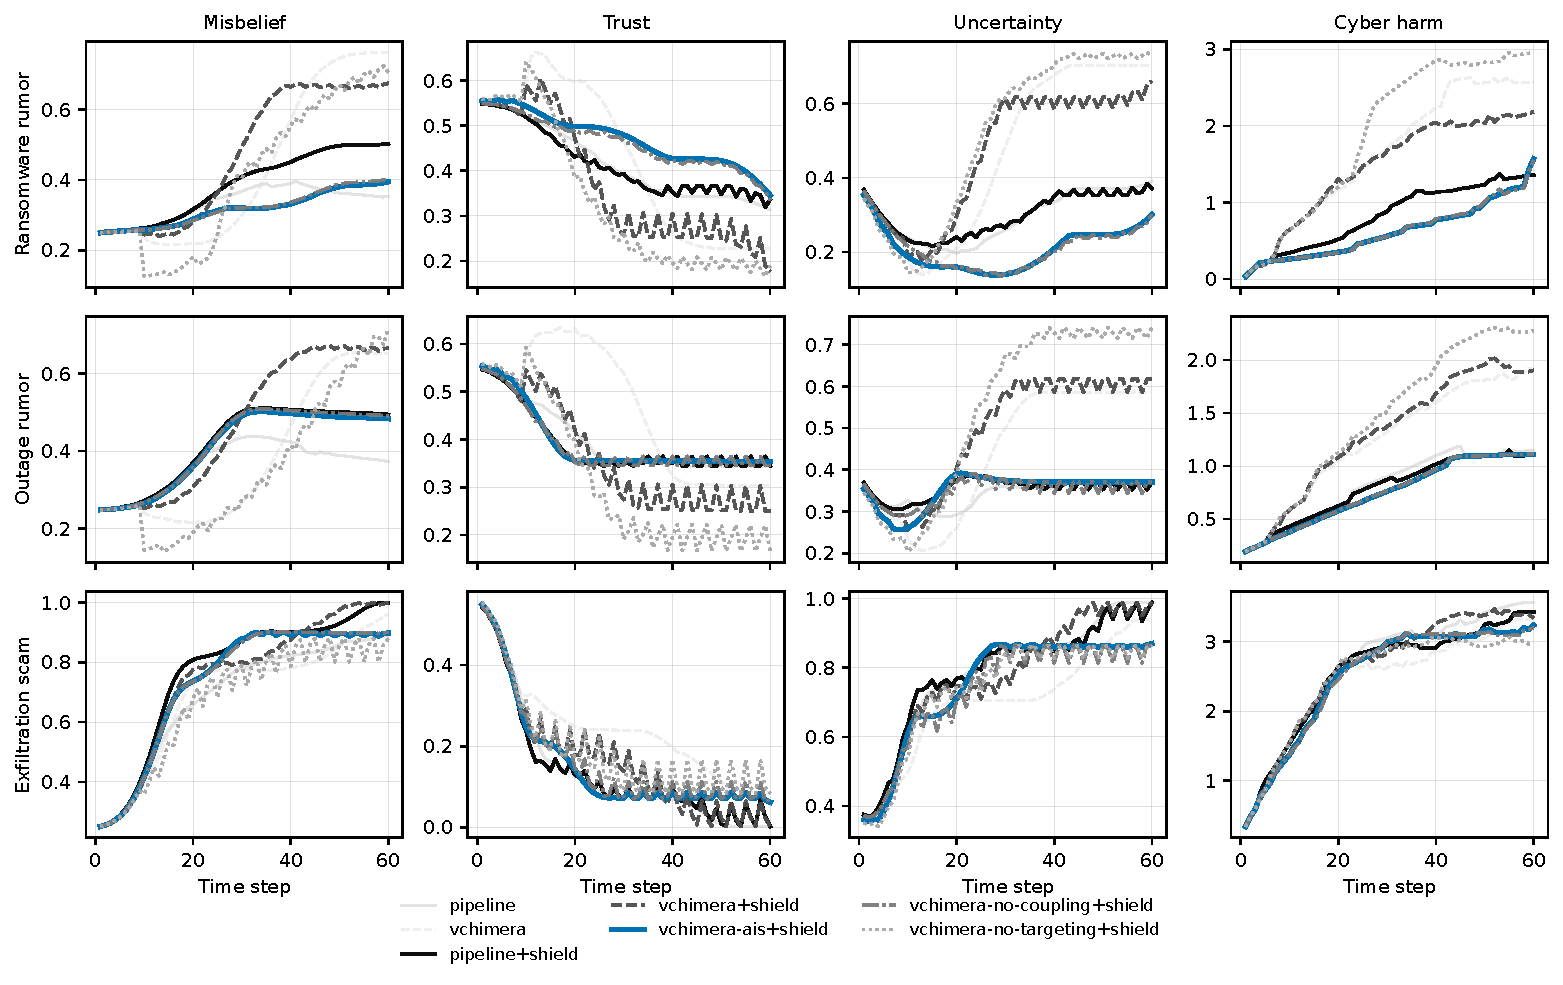
\includegraphics[width=\linewidth]{figures/fig_timeseries_grid_gray.pdf}
  \caption{Time-series dynamics (mean across seeds). Columns: misbelief, trust, uncertainty, cyber harm. Rows: ransomware rumor, outage rumor, exfiltration scam.}
  \label{fig:timeseries_grid}
\end{figure}

\subsection{Robustness and sensitivity}
We perform a grid sensitivity analysis for the \texttt{ransomware\_rumor} scenario under \texttt{vchimera+shield}, varying cyber--social coupling strength and platform moderation effectiveness. Figure~\ref{fig:sensitivity} shows that stronger moderation reliably reduces misbelief, while stronger coupling increases the operational impact of misinformation (amplifying the value of effective communication).

\begin{figure}[t]
  \centering
  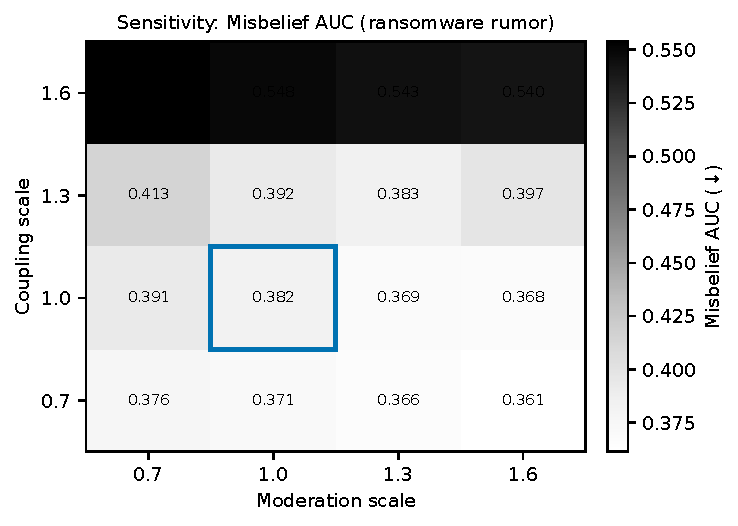
\includegraphics[width=0.85\linewidth]{figures/fig_sensitivity_misbelief_gray.pdf}
  \caption{Sensitivity of misbelief AUC in \texttt{ransomware\_rumor} under \texttt{vchimera+shield} to cyber--social coupling and moderation scales.}
  \label{fig:sensitivity}
\end{figure}

Table~\ref{tab:sensitivity} summarizes outcomes at extreme settings.

\begin{table}[t]
\centering
\caption{Sensitivity summary at extreme settings (\texttt{ransomware\_rumor}, \texttt{vchimera+shield}).}
\label{tab:sensitivity}
\small
\begin{tabular}{lcc}
\toprule
Setting (coupling, moderation) & Misbelief AUC $\downarrow$ & Trust AUC $\uparrow$ \\
\midrule
Low coupling (0.7), high moderation (1.6) & 0.361 & 0.449 \\
High coupling (1.6), low moderation (0.7) & 0.554 & 0.313 \\
\bottomrule
\end{tabular}
\end{table}

\section{Discussion}
Our evaluation supports three qualitative conclusions relevant to socio-technical incident response.

First, coupling communication into operations can help when the cyber--social linkage is strong and correctly specified. In such regimes, the policy can trade operational actions against sentiment dynamics, improving trust and reducing misbelief with limited operational cost. However, when linkage is weak or misspecified, coupling can increase cyber harm. Practical systems should therefore (i) gate coupling on evidence of social-to-cyber impact, (ii) estimate coupling online, or (iii) fall back to a decoupled safe policy when linkage is uncertain.

Second, targeting is valuable when susceptibility is heterogeneous and attention is constrained, but it is not universally dominant. Our ablations suggest that broad counter-messaging can outperform naive targeting in regimes where diffusion rapidly crosses community boundaries or where the model lacks explicit attention/reach constraints. Treating targeting as a tunable design choice---and incorporating empirically grounded segmentation and platform recommender effects---is a key direction for future work.

Third, protocol enforcement is necessary for deployment. Even if an unconstrained policy improves average performance, rare but severe communication failures are unacceptable. The shield provides a clean separation: optimize under soft objectives and enforce hard constraints at runtime, yielding both safety guarantees and auditable intervention logs.

\section{Implications}
For security operations centers and organizational communications units, the results motivate treating crisis communication as an operational control surface rather than an afterthought. Maintaining an explicit sentiment-state estimate (misbelief, trust, uncertainty) enables allocating messaging resources to communities at highest misinformation risk. The protocol shield provides a governance mechanism: organizations can encode policy constraints (e.g., ``do not debunk without evidence'' or ``label uncertainty when uncertainty is high'') and guarantee compliance even when a learned policy proposes unsafe actions. Shield-edit counts and violation logs provide auditable signals for after-action review and continuous improvement of incident playbooks.

At a societal level, verified, evidence-grounded crisis communication can reduce exposure to follow-on scams and avoid overconfident corrections that undermine trust. More broadly, this work illustrates how socio-technical safety mechanisms can be embedded into automated decision systems to protect public trust during disruptive events.

\section{Limitations}
Our study has limitations that motivate future work. The default cyber backend is an abstract incident simulator and omits real-network complexities (legacy constraints, hidden dependencies, and incomplete telemetry). The social ABM is stylized and does not model full language semantics or platform recommender systems. We partially address external validity by exposing parameters, providing calibration tools, and including an adapter scaffold for CybORG, but richer backends and empirical grounding are needed for deployment.

Our baseline policies are intentionally transparent and reproducible. Incorporating learned policies (e.g., MARL) with the same shield may yield stronger performance while retaining guarantees. Finally, trust and belief are represented by proxy variables; real-world use requires careful empirical validation and ethical oversight.

\section{Conclusion}
We introduced \model{}, a misinformation-aware incident response framework that couples cyber operations and crisis communication under explicit protocol constraints. Across scenarios in a coupled cyber--social testbed, the communication shield enforces a hard safety guarantee (zero executed protocol violations) while producing an auditable record of runtime interventions. Effectiveness exhibits scenario-dependent trade-offs: in some regimes the coupled system improves trust and reduces misbelief relative to shielded baselines, while in others naive coupling can increase cyber harm, underscoring that coupling functions and policy weights must be calibrated to operational context. Sensitivity analysis clarifies when verified communication yields the largest marginal value: stronger coupling and weaker moderation increase the operational impact of misinformation, making protocol-safe counter-messaging more consequential. We hope this work stimulates cybersecurity research on closed-loop cyber--social crises and MAS research on verified socio-technical decision systems that align operational effectiveness with governance constraints.

\appendix

\section{Additional dynamics: polarization}
\label{app:polarization}
Polarization trajectories provide a complementary view of social stability beyond misbelief and trust. Figure~\ref{fig:pol_grid} reports polarization over time across the three primary scenarios and the illustrative CybORG transfer run.

\begin{figure}[t]
  \centering
  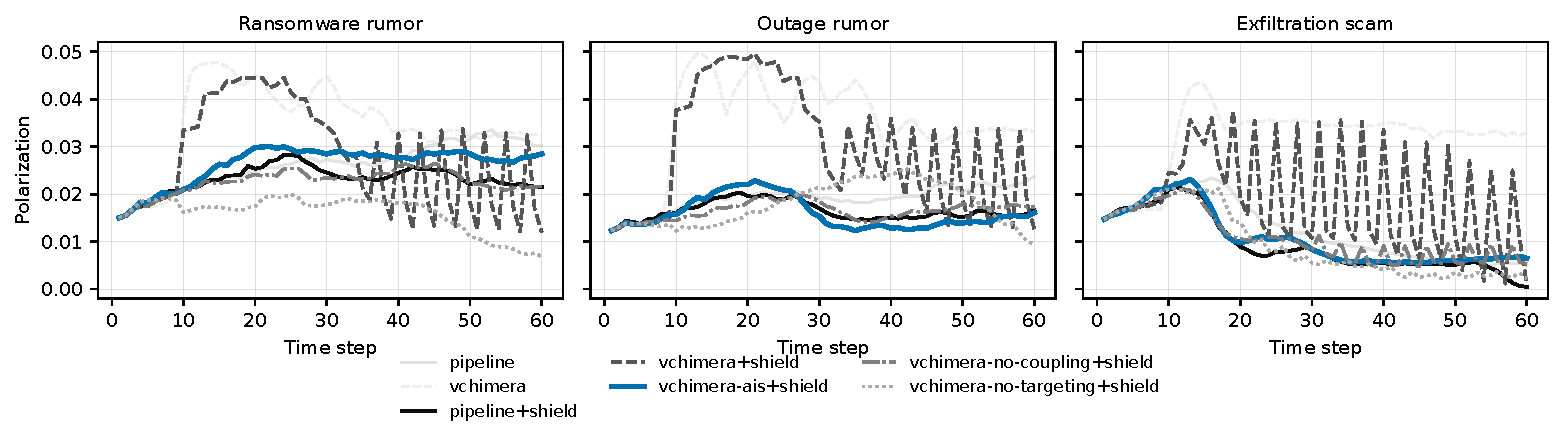
\includegraphics[width=\linewidth]{figures/fig_polarization_grid_gray.pdf}
  \caption{Polarization over time (mean across seeds). Panels correspond to ransomware rumor, outage rumor, exfiltration scam, and the illustrative CybORG transfer run.}
  \label{fig:pol_grid}
\end{figure}

\section{CybORG transfer experiment (artifact extension)}
\label{app:cyborg}
To demonstrate extensibility beyond the default incident backend, the artifact includes an adapter for the CybORG ecosystem \citep{baillie2020cyborg,standen2021cyborg,emerson2024cyborgpp}. CybORG provides a higher-fidelity enterprise-defense setting with richer cyber observations than an abstract attack-graph simulator.

\subsection{Adapter mapping}
The adapter maps CybORG observations (e.g., service availability, detection signals, evidence proxies) into the shared cyber state used by the coupling bus and protocol monitor, enabling the same communication shield and sentiment dynamics to be exercised in the CybORG loop.

\subsection{Illustrative transfer run}
We include an illustrative run on the CC4 enterprise scenario to verify end-to-end integration. Figure~\ref{fig:cyborg_timeseries} reports sentiment trajectories and Figure~\ref{fig:cyborg_polarization_only} reports polarization (mean across seeds in the provided configuration). These results are not intended as a full benchmark comparison; rather, they confirm that \model{} can be coupled to an external cyber-defense backend while maintaining protocol-safe communication.

\begin{figure}[t]
  \centering
  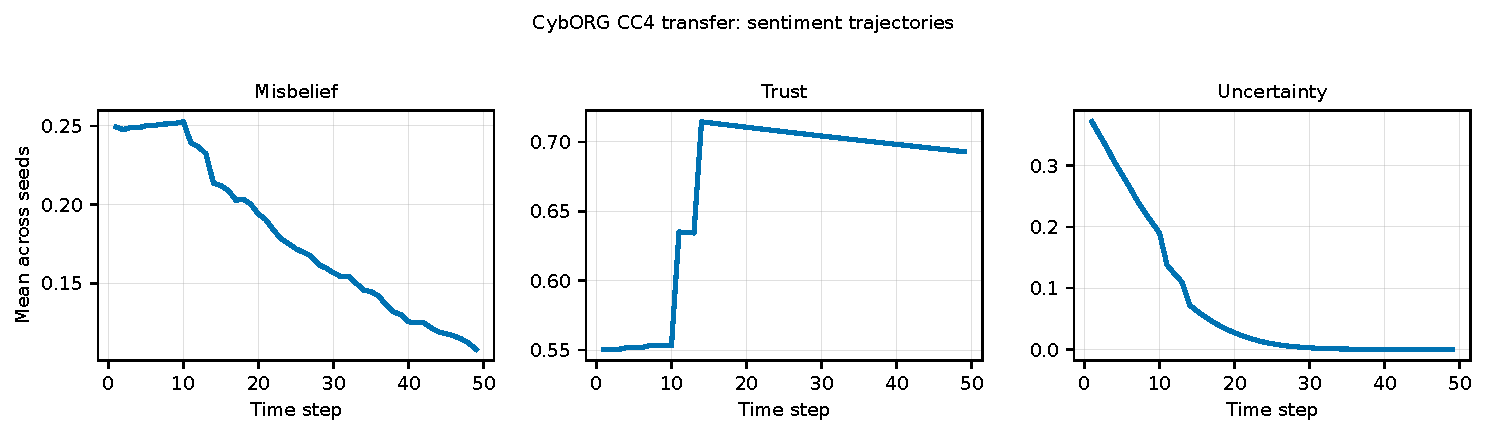
\includegraphics[width=\linewidth]{figures/fig_cyborg_timeseries_grid_gray.pdf}
  \caption{Illustrative CybORG CC4 enterprise transfer run: sentiment trajectories (mean across seeds).}
  \label{fig:cyborg_timeseries}
\end{figure}

\begin{figure}[t]
  \centering
  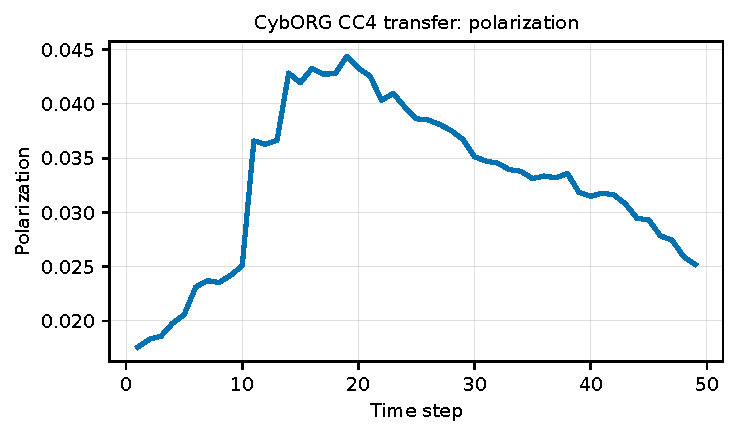
\includegraphics[width=0.8\linewidth]{figures/fig_polarization_cyborg_enterprise_cc4_gray.pdf}
  \caption{Polarization over time for the illustrative CybORG CC4 enterprise transfer run.}
  \label{fig:cyborg_polarization_only}
\end{figure}

\backmatter

\bmhead{Supplementary information}
The accompanying software artifact contains code, configuration files, and scripts to reproduce the experiments, regenerate all figures and tables, and audit protocol-shield interventions. For double-anonymous review, repository identifiers are omitted and should be provided in the submission system or in a camera-ready version.

\bmhead{Abbreviations}
ABM: agent-based model; C-POSG: constrained partially observable stochastic game; MAS: multi-agent systems; MARL: multi-agent reinforcement learning; SOC: security operations center.

\bmhead{Availability of data and materials}
All results reported in this manuscript are generated by simulation. The artifact provides configuration files, deterministic scripts, and raw episode logs enabling regeneration of tables and figures. Links/DOIs should be added upon submission or after de-anonymization.

\bmhead{Code availability}
The \envname{} implementation, experiment pipeline, and analysis scripts are provided as supplementary material / repository artifact (link omitted for review).

\bmhead{Competing interests}
The authors declare no competing interests.

\bmhead{Funding}
Not applicable.

\bmhead{Ethics approval and consent to participate}
Not applicable.

\bmhead{Consent for publication}
Not applicable.

\bmhead{Authors' contributions}
Not applicable for anonymized submission.

\bmhead{Acknowledgements}
Not applicable for anonymized submission.


\bibliography{refs}

\end{document}